%! TeX program = xelatex
\documentclass{article}
\usepackage{amsmath}
\usepackage{amssymb}
\usepackage{fontspec}
\usepackage{graphicx}
\usepackage{hyperref}
\usepackage{tikz}
\usepackage[normalem]{ulem}
\usepackage[margin=0.75in]{geometry}

\graphicspath{{../}, {../../}}
\hypersetup{
  colorlinks   = true,
  urlcolor     = blue,
  linkcolor    = blue,
  citecolor   = red
}

\setmainfont{Noto Serif CJK KR}
\title{5-6. 함수 step C 풀이}
\author{
    \includegraphics[scale=0.25]{logo}
}
\date{}

\begin{document}
\maketitle

\paragraph{1번}
가능한 함수의 개수는 $n^n$개이고, 상수함수의 개수는 $n$개이므로 $f(n) = n^n - n$이다. 또한, 모든 일대일 대응의 개수는 $n!$이고, $x_1$이 $y_3$과 대응되는 경우의 수는 $(n - 1)!$이므로 $g(n) = n! - (n - 1)!$이다. 따라서 $f(4) + g(5) = (4^4 - 4) + (5! - 4!) = 348$이다.

\paragraph{2번}
이 문제는 엄밀하게 가면 정말 어려운 문제이다. \sout{사실 나는 이문제를 제대로 할 자신이 없다. 궁금한 점이 생기면 주변의 수학 월클들께 물어보자.} \newline

문제에서 나왔듯 함수 $f: X \longrightarrow X$는 다음 조건을 만족한다.

\[
    f(\frac{a + b}{2}) = \frac{f(a) + f(b)}{2}
\]

이 식은 함수의 볼록/오목과 관련이 있다. 아마 여러 문제집들이 이 성질을 다룰 텐데, 아무 함수에서 두 점을 찍어서 두 점의 중점 $y$좌표값이 실제 함수값보다 작으면

\[
    f(\frac{a + b}{2}) \le \frac{f(a) + f(b)}{2}
\]

이 함수는 볼록이고, 부등호가 반대가 되면

\[
    f(\frac{a + b}{2}) \ge \frac{f(a) + f(b)}{2}
\]

이 함수는 오목이라고 한다. 문제의 조건을 보면 함수가 볼록도, 오목도 아닌 직선임을 알 수 있고, $f(1) = f(2) = 5$이므로 $f(x) = 5$, 치역의 원소 개수는 \underline{1}이다. \newline

라고 푸는 문제이지만, 아무리 봐도 저 함수의 오목/볼록 조건은 약간 찜찜한 것 같다. 명제 단원에 많이 나오는 ㄱ, ㄴ, ㄷ고르는 문제의 반대 보기처럼, 잘 하면 뚝배기를 깰 수 있을 것처럼 보인다. \sout{응 너만 그래} \newline

\textbf{지금부터는 고1 수학의 범위를 넘어갈 수도 있고, 시험에 거의 100\% 쓸데 없는 내용입니다. 수학을 싫어하시거나, 굳이 깊게 들어가는 것을 노잼이라고 생각하시는 분들은 3번 풀이로 넘어가셔도 됩니다.} 물론 저는 이런 걸 매우 좋아하긴 하지만요. \newline

사실 어떤 함수가 볼록이려면 다음과 같은 조건을 만족해야 한다. ($t$는 0 이상 1 이하의 실수)

\[
    f(tx + (1 - t)y) \le tf(x) + (1 - t)f(y)
\]

자, 그럼 앞서 말한 볼록 함수의 조건

\[
    f(\frac{a + b}{2}) \le \frac{f(a) + f(b)}{2}
\]

이 만족될 때, $f(tx + (1 - t)y) \le tf(x) + (1 - t)f(y)$임을 증명하면 된다. 모든 유리수에 대해 증명하는 것은 간단하다. 위의 식이

\[
    f(\frac{x_1 + x_2 + \cdots + x_k}{k}) \le \frac{f(x_1) + f(x_2) + \cdots + f(x_k)}{k}
\]

와 같음을 보이면 된다. (k는 2 이상의 임의의 양의 정수) 여기서는 \href{https://en.wikipedia.org/wiki/Inequality\_of\_arithmetic\_and\_geometric\_means\#Proof\_by\_Cauchy\_using\_forward\%E2\%80\%93backward\_induction}{코시의 귀납법}이라고 불리는 방법을 사용하겠다.

\subparagraph{$k = 2^n$인 경우} 매우 자명하게 증명할 수 있다. $2^n$개의 항들을 같은 크기의 2조각으로 분할하는 것을 반복하면 된다.

\subparagraph{$2^{k - 1} < k \le 2^k$일 때} $\bar{x} = \frac{x_1 + x_2 + \cdots + x_3}{k}$라고 하면,

\[
    f(\bar{x}) = f(\frac{x_1 + x_2 + \cdots + x_k + \bar{x} + \cdots + \bar{x}}{2^n}) \le \frac{f(x_1) + f(x_2) + \cdots + f(x_k) + (2^n - k)f(\bar{x})}{2^n}
\]

여기서 $kf(\bar{x}) \le f(x_1) + \cdots + f(x_k)$임을 알 수 있다. \newline

그렇다면, 모든 실수에 대해 성립하는지는 어떻게 알 수 있을까? \sout{월 6, 7교시 수학을 수강하는 친구들은 내가 이걸 증명하려다 망한 것을 보았을 것이다.} 사실, 이 질문에 대한 답은 단순하다. 위의 조건은 $f$가 연속이라는 가정이 숨어 있다. 모든 유리수에 대해 성립하므로, 연속성에 의해 모든 실수에 대해서도 성립하는 것이다. 고1 수준에서는 불연속인 함수를 다룰 일이 거의 없고, 다룬다 하더라도 오목/볼록을 따지지는 않으므로 이러한 가정이 보이지 않았던 것 뿐이다.

\paragraph{3번}

\subparagraph{보기 ㄱ} $f$, $g$가 모두 항등함수이면 성립함은 당연하다.
\subparagraph{보기 ㄴ} $f$와 $g$가 역함수 관계일 수도 있다.
\subparagraph{보기 ㄷ} $f$와 $g$가 모두 일대일대응이어도 상관 없다. \newline

따라서 참인 것은 ㄱ, 따라서 정답은 \underline{1}이다.

\paragraph{4번}
$y = f(x)$일 때, $f(y) = x$이므로 $f(f(x)) = x$의 서로 다른 실근 개수는 $y = f(x)$와 $x = f(y)$의 교점 개수와 같다.

\begin{center}
    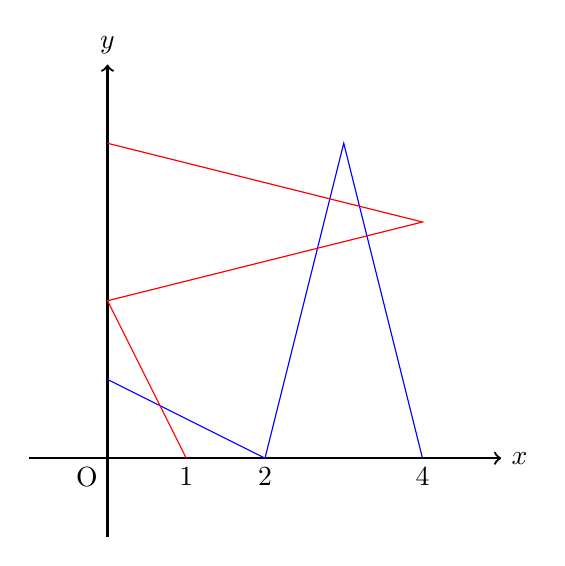
\begin{tikzpicture}
        \draw[thick,->] (-1, 0) -- (5, 0) node[anchor=west] {$x$};
        \draw[thick,->] (0, -1) -- (0, 5) node[anchor=south] {$y$};
        \draw[blue] (0, 1) -- (2, 0) -- (3, 4) -- (4, 0);
        \draw[red] (1, 0) -- (0, 2) -- (4, 3) -- (0, 4);
        \node[anchor=north east] at (0, 0) {$\mathrm{O}$};
        \node[anchor=north] at (1, 0) {$1$};
        \node[anchor=north] at (2, 0) {$2$};
        \node[anchor=north] at (4, 0) {$4$};
    \end{tikzpicture}
\end{center}

그림에서 볼 수 있듯 두 그래프의 교점은 5개이고, 따라서 정답은 \underline{5}이다.

\paragraph{5번}
그래프를 통해 $g(x) = -x + 1$임을 알 수 있다. 역함수를 구하면 $g^{-1}(x) = -x + 1$이고, 따라서 $y = (g^{-1} \circ f)(x) = -f(x) + 1$를 그래프로 그리면 다음과 같다.

\begin{center}
    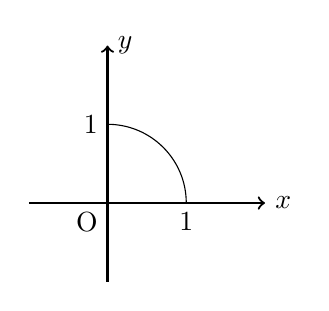
\begin{tikzpicture}
        \draw[thick,->] (-1, 0) -- (2, 0) node[anchor=west] {$x$};
        \draw[thick,->] (0, -1) -- (0, 2) node[anchor=west] {$y$};
        \draw (1,0) arc (0:90:1);
        \node[anchor=north east] at (0, 0) {$\mathrm{O}$};
        \node[anchor=north] at (1,0) {$1$};
        \node[anchor=east] at (0,1) {$1$};
    \end{tikzpicture}
\end{center}
\end{document}
